%%% ===================================================================
%%% RCS Header:
%%% $RCSfile: local.el,v $
%%% $Revision: 1.27 $
%%% $Date: 2014/11/07 15:36:00 $
%%% $Author: backofen $
%%% $Locker:  $
%%% ===================================================================

\section{\texorpdfstring{$\mathcal{O}$}{O}-Notation}

\toclesssubsection{Motivation / Definition}

\begin{frame}{$\mathcal{O}$-Notation}{Motivation}
  \textbf{We are interested in:}
  \begin{itemize}
  \item example sorting:
    \begin{itemize}
      \item
        Runtime of \textit{Minsort} ``is growing as" $\quad{}\quad{}n^2$
      \item
         Runtime of \textit{HeapSort} ``is growing as'' $\quad{}n \, \log n$
    \end{itemize}
    \item<2->
      Growth of a function in runtime $T(n)$
      \begin{itemize}
      \item The role of constants (e.g. $1ns$) is minor
      \item it is enough if relation holds for some $n\geq \ldots$
      \end{itemize}
    \item<3->
      Describe the growth of the function \textbf{more formally}
    \begin{itemize}
      \item
        By the means of Landau-Symbols \cite{wikipedia_big_o_notation}):
            \begin{itemize}
                \item
                    {\color{Mittel-Blau}$\mathcal{O}(n)$} (Big O of $n$),
                \item
                    {\color{Mittel-Blau}$\Omega (n)$} (Omega of $n$),
                \item
                    {\color{Mittel-Blau}$\Theta (n)$} (Theta of $n$)
            \end{itemize}
    \end{itemize}
  \end{itemize}
\end{frame}

%-------------------------------------------------------------------------------

\begin{frame}{$\mathcal{O}$-Notation}{Definition}
  \textbf{Big $\mathcal{O}$-Notation:}
  \begin{itemize}
    \item
     Consider the function:
      $f\!: \mathbb{N} \to \mathbb{R}, \; n \mapsto f(n)$
      \begin{itemize}
        \item
          $\mathbb{N}\!:$ Natural numbers $\rightarrow$ input size
        \item
          $\mathbb{R}\!:$ Real numbers $\rightarrow$ runtime
      \end{itemize}
   \item
     \textbf{Example:}
   \begin{itemize}[<+->]
     \item
       $f(n) = 3 \, n$
     \item
       $f(n) = 2 \, n \, \log n$
     \item
       $f(n) = \frac{1}{10} n^2$
     \item
       $f(n) = n^2 + 3 \, n \, \log n - 4 \, n$
    \end{itemize}
  \end{itemize}
\end{frame}

%-------------------------------------------------------------------------------

\begin{frame}{$\mathcal{O}$-Notation}{Definition}
  \textbf{Big $\mathcal{O}$-Notation:}
  \begin{itemize}
    \item
      Given two functions $f$ and $g$: \\
      $f,g\!: \mathbb{N} \to \mathbb{R}$
    \item
      \textbf{Intuitive:} $f$ is Big-O from $g$ ($f$ is $\mathcal{O}(g)$)\\
         \begin{itemize}
            \item
            ... if $f$ relative to $g$ does not grow faster than $g$
            \item
                the growth rate matters, not the absolute values
        \end{itemize}
  \end{itemize}
\end{frame}


%-------------------------------------------------------------------------------
\usetikzlibrary{arrows,shapes}
% For every picture that defines or uses external nodes, you'll have to
% apply the 'remember picture' style. To avoid some typing, we'll apply
% the style to all pictures.
\tikzstyle{every picture}+=[remember picture]

% By default all math in TikZ nodes are set in inline mode. Change this to
% displaystyle so that we don't get small fractions.
%\everymath{\displaystyle}

\tikzstyle{na} = [baseline=-.5ex]

\begin{frame}{$\mathcal{O}$-Notation}{Definition}
  \textbf{Big $\mathcal{O}$-Notation:}%
  \begin{itemize}
    \item
      \textbf{Informal:} $f = \mathcal O(g)$\\
      
        \begin{itemize}
            \item
               $=$ corresponds to $is$ not $is equal$
            \item
               ... if for some value $n_0$ for all $n \geq n_0$
            \item
               $f(n) \leq C \cdot g(n)$ for a constant C
            \item 
                ($f = \mathcal O(g)$: From a value $n_0$ for all $n \geq n_0 \rightarrow f(n) \leq C \cdot g(n)$)
        \end{itemize}
  \end{itemize}
  \begin{block}{\textbf{Formal:} $f \in \mathcal O(g)$}
    \begin{math}
      \mathcal O(g) = \lbrace \tikz[baseline] {\node (fun) [anchor=base] {f};}: \mathbb{N} \to \mathbb{R} ~ \tikz[baseline] {\node (for) [anchor=base] {|};}\tikz[baseline] {\node (exone) [anchor=base] {$\exists$};}\!\!n_0 \in \mathbb{N},\tikz[baseline] {\node (extwo) [anchor=base] {$\exists$};}\!\!C > 0,\tikz[baseline] {\node (forall) [anchor=base] {$\forall$};}\!\!n > n_0\!\!\tikz[baseline] {\node (such) [anchor=base] {:};}        f(n) \leq C \cdot g(n)\rbrace
    \end{math}
  \end{block}
\tikz[baseline] {\node (funtext) [anchor=base] {
{\footnotesize\onslide<2->{\begin{tabular}[c]{@{}c@{}}
      ``set of\\
      all functions''
    \end{tabular}}
}};}\quad{} \tikz[baseline] {\node (fortext) [anchor=base] {
{\footnotesize\onslide<3->{\begin{tabular}[c]{@{}c@{}}
    ``for which''
    \end{tabular}}
}};}\quad{} \tikz[baseline] {\node (extext) [anchor=base] {
{\footnotesize\onslide<4->{\begin{tabular}[c]{@{}c@{}}
    ``it exists''
    \end{tabular}}
}};}\quad{} \tikz[baseline] {\node (foralltext) [anchor=base] {
{\footnotesize\onslide<5->{\begin{tabular}[c]{@{}c@{}}
    ``for all''
    \end{tabular}}
}};}\quad{} \tikz[baseline] {\node (suchtext) [anchor=base] {
{\footnotesize\onslide<6->{\begin{tabular}[c]{@{}c@{}}
    ``such that''
    \end{tabular}}
}};}
\begin{tikzpicture}[>=stealth,overlay,thick]
        \path[->,color=red]<2-> (funtext) edge [bend left]  (fun);
        \path[->,color=red]<3-> (fortext) edge [bend left]  (for);
        \path[->,color=red]<4-> (extext) edge [bend left]  (exone);
        \path[->,color=red]<4-> (extext) edge [bend right]  (extwo);
        \path[->,color=red]<5-> (foralltext) edge [bend left]  (forall);
        \path[->,color=red]<6-> (suchtext) edge [bend left]  (such);
\end{tikzpicture}

\end{frame}

%-------------------------------------------------------------------------------

\subsection{Examples}

\begin{frame}{$\mathcal{O}$-Notation}{Examples}
  \textbf{Illustration of the Big O-Notation:}\\[-1.0em]
  \begin{columns}
    \begin{column}{0.9\textwidth}
      \begin{figure}[!h]
        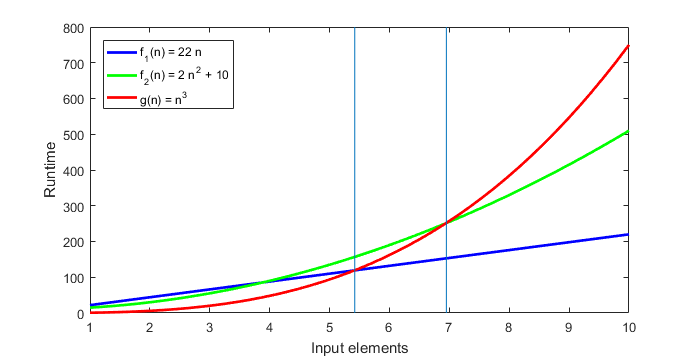
\includegraphics[width=\linewidth]{Images/BigONotationRuntime.png}
        \caption{Runtime of two algorithms $f_1, f_2$}
        \label{fig:big_o_runtime_example}
      \end{figure}
    \end{column}
    \begin{column}{0.1\textwidth}
      \vspace{-4.75em}\\
      \hspace*{-2.5em}$g(n)$\\[2.0em]
      \hspace*{-2.5em}$f_2 \in \mathcal{O}(g)$\\[2.5em]
      \hspace*{-2.5em}$f_1 \in \mathcal{O}(g)$
    \end{column}
  \end{columns}
\end{frame}

%-------------------------------------------------------------------------------

\begin{frame}{$\mathcal{O}$-Notation}{Examples}
  \textbf{Example:}
  \begin{itemize}
    \item
      $f(n) = 5 \, n + 7, \; g(n) = n$\\
      $\Rightarrow$ $5 \, n + 7 \in \mathcal{O}(g)$\\
      $\Rightarrow f \in \mathcal{O}(g)$
     \item
      \textbf{Intuitive:}\\
      $f(n) = 5 \, n + 7$ $\rightarrow$ linear growth
  \end{itemize}
  \begin{alertblock}{Attention}
    $f(n) \leq g(n)$ is not correct, better is
    $f(n) \leq C \cdot g(n) \;\; \forall n > n_0$.
  \end{alertblock}
\end{frame}

%-------------------------------------------------------------------------------

\begin{frame}{$\mathcal{O}$-Notation}{Proof}
  \begin{proof}[
    We have to proof:
    \begin{math}
      \exists n_0, \, \exists C, \, \forall n \geq n_0 \! : \;
        5 \, n + 7 \leq C \cdot n
    \end{math}
  ]
    \begin{eqnarray*}
\onslide<2->{      &5 \, n + 7 &\leq \;\; 5 \, n + n \hspace{1em} (\text{for} ~ n \geq 7)}\\
\onslide<3->{          && \leq \;\; 6 \, n}
    \end{eqnarray*}
\onslide<4->{    $\hspace{1.5em} \Rightarrow n_0 = 7, \, C = 6$ \qedhere}
  \end{proof}
\end{frame}

%-------------------------------------------------------------------------------

\begin{frame}{$\mathcal{O}$-Notation}{Proof}
  \begin{proof}[Alternate proof:]
    \begin{eqnarray*}
\onslide<2->{       &5 \, n + 7 &\leq \;\; 5 \, n + 7 \, n \hspace{1em} (\text{for} ~ n \geq 1)}\\
\onslide<3->{       && \leq \;\; 12 \, n }
    \end{eqnarray*}
    \onslide<4->{$\hspace{1.5em} \Rightarrow n_0 = 1, \, C = 12$ \qedhere}
  \end{proof}
\end{frame}

%-------------------------------------------------------------------------------

\begin{frame}{$\mathcal{O}$-Notation}{Examples}
  \textbf{Big O-Notation:}
  \begin{itemize}
    \item
      We are only interested in the term with the Highest-order, the fasted growing Summand,
      the others will be ignored
    \item
      $f(n)$ is limited {\color{Mittel-Blau}from above} by $c \cdot g(n)$
  \end{itemize}
  \textbf{Examples:}
  \begin{align*}
     2 \, n^2 + 7 \, n - 20 \in & \,\mathcal{O}(n^2) \\
     2 \, n^2 + 7 \, n \, \log n - 20 \in & {}\\
     7 \, n \, \log n - 20 \in & {}\\
     5 \in & {}\\
     2 \, n^2 + 7 \, n \, \log n + n^3 \in & {}\\
  \end{align*}
\end{frame}

\begin{frame}{Harder Example}
  \begin{itemize}
  \item polynomes are simple
  \item more problematic: combination of complex functions
    \begin{displaymath}
           2 \sqrt{x} + 3 \ln x \in \mathcal{O} (??)
    \end{displaymath}
  \end{itemize}
\end{frame}
%-------------------------------------------------------------------------------

\section{\texorpdfstring{$\Omega$}{Omega}-Notation}

\begin{frame}{$\Omega$-Notation}{Definition}
  \textbf{Omega-Notation:}
  \begin{itemize}
    \item
      \textbf{Intuitive}:\\

          \begin{itemize}
            \item
              $f \in \Omega(g)$, $f$ is growing at least as fast as $g$
            \item
              So the same as Big-O but with \textit{at-least} and not \textit{at-most}.
          \end{itemize}

  \end{itemize}
 	\begin{block}{\textbf{Formal:} $f \in \Omega(g)$}
    \begin{math}
      \Omega(g) = \lbrace f: \mathbb{N} \to \mathbb{R} ~ | ~
        \exists n_0 \in \mathbb{N}, \, \forall n > n_0, \, \exists C > 0: \,
        f(n) \tikz[baseline] {\node (geq) [anchor=base] {$\geq$};} C \cdot g(n)\rbrace
    \end{math}
 	\end{block}
        \begin{center}
          \tikz[baseline] {\node (geqtext) [anchor=base] {
{\footnotesize\onslide<1->{\begin{tabular}[c]{@{}c@{}}
      ``in $O(n)$\\
      we had $\leq$''
    \end{tabular}}
}};}
 \end{center}
\begin{tikzpicture}[>=stealth,overlay,thick]
  \path[->,color=red] (geqtext) edge [bend right]  (geq);
\end{tikzpicture}
\end{frame}

%-------------------------------------------------------------------------------

\begin{frame}{$\Omega$-Notation}{Proof}
  \begin{proof}[Proof of $f(n) = 5n + 7 \in \Omega(n)$:]
    \begin{eqnarray*}
      &\underbrace{5 \, n + 7}_{f(n)} &\geq \;\; \underbrace{1 \cdot n}_{g(n)}
      \hspace{1em} (\text{for} ~ n \geq 1)
    \end{eqnarray*}
    $\hspace{1.5em} \Rightarrow n_0 = 1, \, C = 1$ \qedhere
  \end{proof}
\end{frame}

%-------------------------------------------------------------------------------

\begin{frame}{$\Omega$-Notation}{Examples}
  \textbf{Illustration of the Omega-Notation:}\\[-1.0em]
  \begin{columns}
    \begin{column}{0.9\textwidth}
      \begin{figure}[!h]
        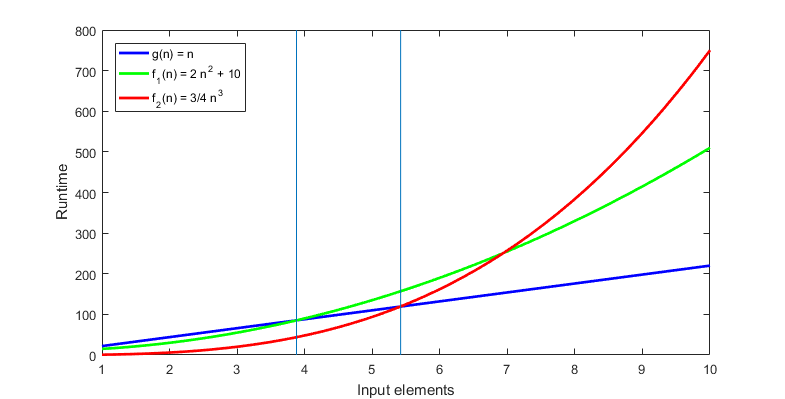
\includegraphics[width=\linewidth]{Images/OmegaNotationRuntime.png}
        \caption{Runtime of two algorithms $f_1, f_2$}
        \label{fig:omega_o_runtime_example}
      \end{figure}
    \end{column}
    \begin{column}{0.1\textwidth}
      \vspace{-4.75em}\\
      \hspace*{-2.5em}$f_2 \in \Omega(g)$\\[2.0em]
      \hspace*{-2.5em}$f_1 \in \Omega(g)$\\[2.5em]
      \hspace*{-2.5em}$g(n)$
    \end{column}
  \end{columns}
\end{frame}

%-------------------------------------------------------------------------------

\begin{frame}{$\Omega$-Notation}{Examples}
  \textbf{Big Omega-Notation:}
  \begin{itemize}
    \item
      We are only interested in the term with the Highest-order, the fasted growing Summand,
      the others will be ignored.
    \item
      $f(n)$ is limited {\color{Mittel-Blau}from underneath} by
      $c \cdot g(n)$.\\
  \end{itemize}
  \textbf{Examples:}
  \begin{align*}
    2 \, n^2 + 7 \, n - 20 \in & \,\Omega(n^2)\\
    2 \, n^2 + 7 \, n \, \log n - 20 \in & {}\\
    7 \, n \, \log n - 20 \in & {}\\
    5 \in & {}\\
    2 \, n^2 + 7 \, n \, \log n + n^3 \in & {}
  \end{align*}
\end{frame}

%-------------------------------------------------------------------------------

\section{\texorpdfstring{$\Theta$}{Theta}-Notation}

\begin{frame}{$\Theta$-Notation}{Definition}
  \textbf{Theta-Notation:}
  \begin{itemize}
    \item
      \textbf{Intuitive}: $f$ is Theta from $g$ ...\\
        \begin{itemize}
            \item
              ... if $f$ is growing as much as $g$
            \item
              $f \in \Theta(g)$, $f$ is growing at the same speed as $g$
       \end{itemize}
  \end{itemize}
 	\begin{block}{\textbf{Formal:} $f \in \Theta(g)$}
 		$\Theta(g) = \underbrace{\mathcal O(g) \cap \Omega(g)}_{Intersection}$
 	\end{block}
  \textbf{Example:}\\
  \hspace*{1.5em}$f(n) = 5 \, n + 7, \;
    f(n) \in \mathcal{O}(n), \,
    f(n) \in \Omega(n)$\\
  \hspace*{3.0em}$\Rightarrow f(n) \in \Theta(n)$\\[0.5em]
  \begin{center}
   \textit{Proof for $\mathcal{O}(g)$ and $\Omega(g)$ look at slides 14 and 19}
  \end{center}
\end{frame}

\begin{frame}{$\Theta$-Notation}{Graphs}
     \begin{center}
       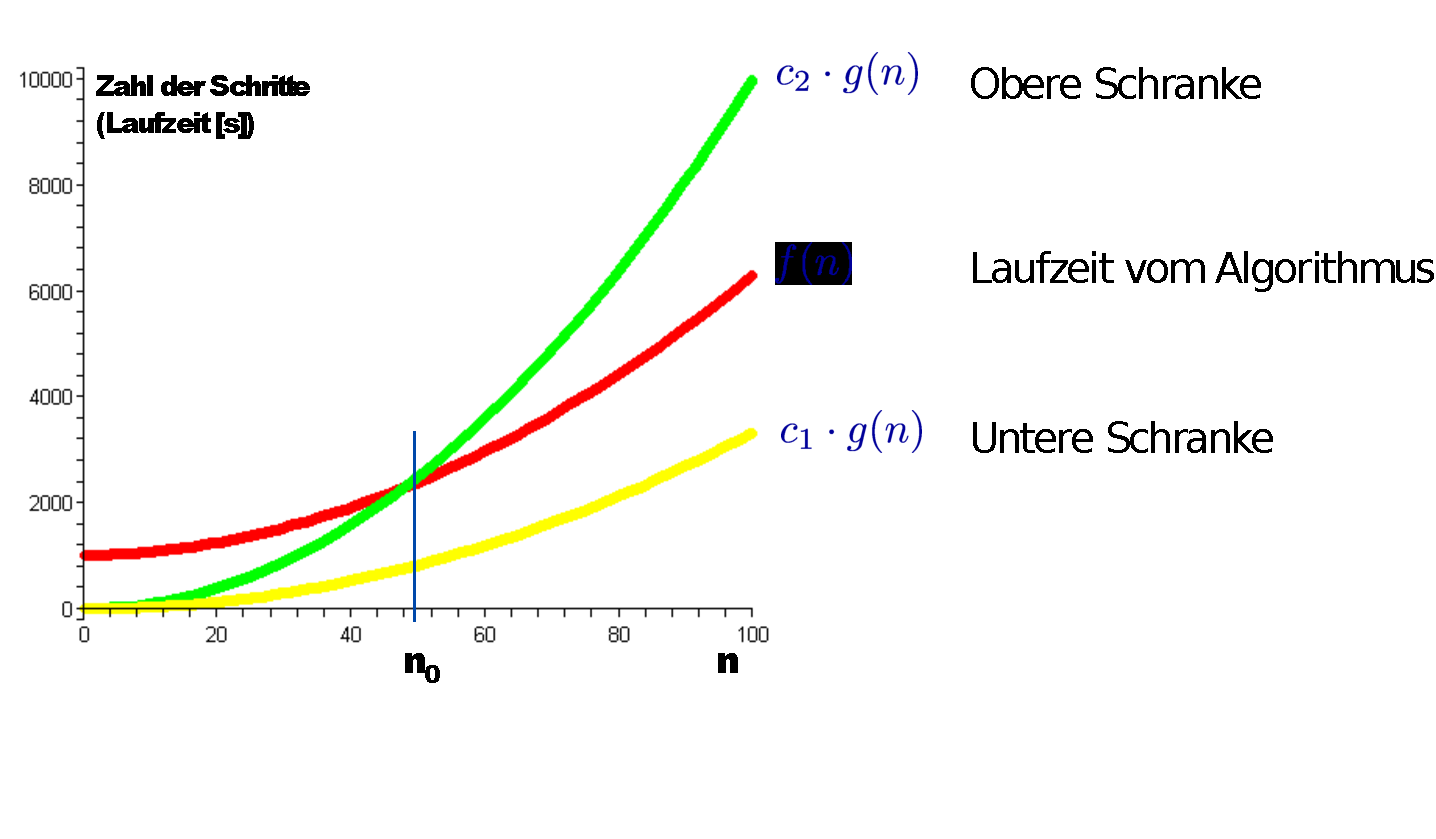
\includegraphics[width=0.8\textwidth]{Images/runtime-theta.pdf}
  \end{center}
  \begin{itemize}
  \item $f$ and $g$ have the same ``growth''
  \end{itemize}
\end{frame}
%-------------------------------------------------------------------------------

\section{Runtime}

\toclesssubsection{Summary}

\begin{frame}{Runtime}{Landau-Symbol Summary}
  \textbf{Big O-Notation} $\mathcal{O}(n)$\textbf{:}\\
    \begin{itemize}
      \item
        $f$ is growing {\color{Mittel-Blau}at least} as fast as $g$
      \item
        $C \cdot g(n)$ is the upper bound
    \end{itemize}
  \textbf{Big Omega-Notation} $\Omega(n)$\textbf{:}\\
  \begin{itemize}
    \item
      $f$ is growing {\color{Mittel-Blau}at maximum} as fast as $g$
    \item
      $C \cdot g(n)$ is the lower bound
  \end{itemize}
  \textbf{Big Theta-Notation} $\Theta(n)$\textbf{:}\\
  \begin{itemize}
    \item
      $f$ is growing at {\color{Mittel-Blau}the same} speed as $g$
      \begin{itemize}
        \item
          $C_1 \cdot g(n)$ is the lower bound
        \item
          $C_2 \cdot g(n)$ is the upper bound
      \end{itemize}
  \end{itemize}
\end{frame}

%-------------------------------------------------------------------------------

\begin{frame}{Runtime}{Common Runtimes}
  \begin{table}[!h]
    \begin{center}
      \caption{Common runtime types}
      \label{RuntimeTable}
      \begin{tabularx}{\textwidth}{XX}
        Runtime & Growth\\
        \hline
        $f \in \Theta (1)$ & constant time\\
        $f \in \Theta (\log n) = \Theta (\log_k n)$ & logarithmic time\\
        $f \in \Theta (n)$ & linear time\\
        $f \in \Theta (n \, \log n)$ & n-log-n time (nearly linear)\\
        \hline
        $f \in \Theta (n^2)$ & squared time\\
        $f \in \Theta (n^3)$ & cubic time\\
        $f \in \Theta (n^k)$ & polynomial time\\
        \hline
        $f \in \Theta (k^n)$, $f \in \Theta(2^n)$ & exponential time
      \end{tabularx}
    \end{center}
  \end{table}
\end{frame}

%-------------------------------------------------------------------------------

\subsection{Limit / Convergence}

\begin{frame}
  \begin{itemize}
  \item so far: 
    \begin{itemize}
    \item membership in $O(\ldots)$ proofed \textbf{manually}
      \begin{center}
        explicit calculation of $n_0$ and $C$
      \end{center}
    \item \textbf{however:} both reminds of \textbf{limits} in calculus
    \end{itemize}
  \end{itemize}
\end{frame}

\begin{frame}{$\mathcal{O}$-Notation}{Limit / Convergence}
  \textbf{Definition of \enquote{Limit}}
  \begin{itemize}
    \item
      The limit of an indefinite sequence $f_1, f_2, f_3$... is $L$\\
      if for all $\epsilon > 0$ one $n_0 \in \mathbb{N}$ exists, such that for all \\
      $n \geq n_0$ the following holds true: $\Vert f_n - L \Vert \leq \epsilon$
    \item
      A function $f\!: \mathbb{N} \rightarrow \mathbb{R}$ can be written as a
      sequence\\
      $\Rightarrow$ $\lim\limits_{n \rightarrow \infty}$ $f_n$ = $L$
  \end{itemize}
  \begin{block}<2->{Convergence}
    \begin{math}
      \forall \epsilon > 0 \; \exists n_0 \in \mathbb{N} \;\;
      \forall n \geq n_0 \! : \; \Vert f_n - L \Vert \leq \epsilon
    \end{math}
  \end{block}
\end{frame}

%-------------------------------------------------------------------------------

\begin{frame}{$\mathcal{O}$-Notation}{Limit / Convergence}
  \begin{itemize}
  \item Example for a limit proof
  \item function $f(n) = 2 + \frac{1}{n}$ with limes $2$
  \item ``engineering'' solution: use $n=\infty{}$
    \begin{displaymath}
      \frac{1}{\infty}=0 \Rightarrow       \lim_{n \to \infty} f(n)
        = \lim_{n \to \infty} 2 + \dfrac{1}{n}
        = 2
    \end{displaymath}
  \end{itemize}
\end{frame}
\begin{frame}{$\mathcal{O}$-Notation}{Limit / Convergence}
  \begin{itemize}
  \item Now a more formal proof for $\displaystyle\lim_{n \to \infty} 2 +
    \dfrac{1}{n}  = 2$
  \item we need to show: for all given $\epsilon$ there is an $n_0$ such
    that for all $n \geq n_0$
    \begin{displaymath}
      \left| 2 + \dfrac{1}{n} - 2 \right| =  \left| \dfrac{1}{n}  \right| \leq \epsilon
    \end{displaymath}
  \item<2-> e.g.: for $\epsilon=0.01$ we get $\frac{1}{n} \leq \epsilon$
    for $n\geq 100$
  \item<3-> in general
    \begin{displaymath}
      n_0 = \left\lceil \dfrac{1}{\epsilon} \right\rceil
    \end{displaymath}
  \item<4-> then we get:
    \begin{eqnarray*}
      \left|
        \frac{1}{n} \vphantom{\dfrac{1}{\frac{1}{\epsilon}}}
      \right|
        = \dfrac{1}{n}
      \; \leq \;
      \dfrac{1}{n_0} =  \dfrac{1}{\left\lceil\frac{1}{\epsilon}
        \right\rceil}
\leq   \dfrac{1}{\frac{1}{\epsilon}}
        = \epsilon
      \qed
    \end{eqnarray*}
  \end{itemize}
\end{frame}

%-------------------------------------------------------------------------------

\begin{frame}{$\mathcal{O}$-Notation}{Limit / Convergence}
  Let $f,g \! : \; \mathbb{N} \to \mathbb{R}$ with an existing limit
  \[\lim_{n \to \infty} \dfrac{f(n)}{g(n)} = L\]
  So we can say:
  \begin{align}
    & f \in \mathcal{O}(g) & \Leftrightarrow
    && \lim_{n \to \infty} \dfrac{f(n)}{g(n)} < \infty\\
    & f \in \Omega(g) & \Leftrightarrow
    && \lim_{n \to \infty} \dfrac{f(n)}{g(n)} > 0\\
    & f \in \Theta(g) & \Leftrightarrow
    && 0 < \lim_{n \to \infty} \dfrac{f(n)}{g(n)} < \infty
  \end{align}
\end{frame}

%-------------------------------------------------------------------------------

\begin{frame}{$\mathcal{O}$-Notation}{Limit / Convergence}
  \[
    f \in \mathcal{O}(g)
    \; \Leftrightarrow \;
    \lim\limits_{n \rightarrow \infty} \frac{f(n)}{g(n)} < \infty
  \]
  \begin{proof}[Forward proof ($\Rightarrow$):]
     $f \in \mathcal{O}(g) \stackrel{\text{def. of }\mathcal{O}(n)}{\Rightarrow}
     \exists n_0, \, C\; \forall n \geq n_0:
     \; f(n) \leq C \cdot g(n)$
     \begin{alignat*}{2}
       \Rightarrow && \exists n_0, \, C\; \forall n \geq n_0: \dfrac{f(n)}{g(n)} &\leq \; C\\
       \Rightarrow && \displaystyle
       \lim_{n \to \infty}\dfrac{f(n)}{g(n)} &\leq \; C
       \qedhere
      \end{alignat*}
  \end{proof}
\end{frame}

%-------------------------------------------------------------------------------

\begin{frame}{$\mathcal{O}$-Notation}{Limit / Convergence}
  \begin{proof}[Backward proof ($\Leftarrow$):]
    \begin{center}
      \vspace{-0.5em}
      \begin{math}
        \begin{aligned}
          & {} & \lim_{n \to \infty} \frac{f(n)}{g(n)} &< \; \infty\\
          & \Rightarrow & \lim_{n \to \infty} \frac{f(n)}{g(n)} &= \; C &&
          \hspace*{1.5em}\text{For some } C \in \mathbb{R} \text{ (Limit)}
        \end{aligned}
      \end{math}
      \vspace{1.0em}\\
      \begin{math}
        \begin{aligned}
          \stackrel{\text{def. limes}}{\Rightarrow} \hspace*{0.5em} &&
          \exists n_0, \, \forall n \geq n_0: \hspace*{1.0em}&&
          \frac{f(n)}{g(n)} &\leq \; C + \varepsilon \;\;\; (e.g.\;\varepsilon = 1)\\
          \Rightarrow \; &&
          \exists n_0, \, \forall n \geq n_0: \hspace*{1.0em}&&
          f(n) &\leq \; \underbrace{(C + 1)}_{O-notation\;constant} \cdot g(n)\\
          \Rightarrow \; &&
          f \in \mathcal{O}(g)
          \qedhere
        \end{aligned}
      \end{math}
    \end{center}
  \end{proof}
\end{frame}

%%% ==========================================
%%% This should be at the END of the file !!!!!!
%%%
%%% Local Variables: 
%%% mode: latex 
%%% TeX-master: "~/TeX/TeXinput/Scripts/Algo-Data-EMS/Rolf-2016/AlgoDat/Lecture-3/Lecture.tex" 
%%% End: 
%%% ==========================================
